\subsubsection{Wavelength estimation}
\label{introReceiver}
Laser wavelength is one of the most important parameters influencing the whole design of photon detection device and \acs{laser} emitter choosing. Different emitter wavelengths have different photon detection efficiency or probability to photon receiver. To choose which type of \acs{laser} is feasible, it is best to start with which wavelength the receiver can detect.

According to the photon detection probability distribution diagram for \acs{SPAD} and \acs{MPD} in figure \ref{fig:SPAD_efficiency} and \ref{fig:MPD_efficiency}, the general most sufficient wavelength range is between 400nm to 900nm. 

\begin{figure}
\centering
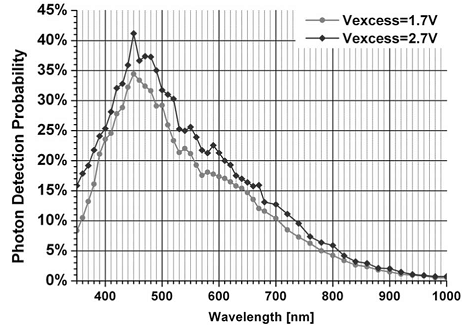
\includegraphics[scale=1]{chapters/img/SPAD_efficiency.png}
\caption{\acs{SPAD} photon detection probability as a function of wavelength for two values of excess bias voltage}
\label{fig:SPAD_efficiency}
\end{figure}

\begin{figure}
\centering
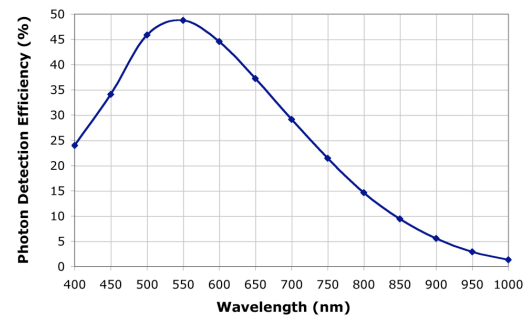
\includegraphics[scale=1]{chapters/img/MPD_efficiency.png}
\caption{\acs{MPD} photon detection probability as a function of wavelength}
\label{fig:MPD_efficiency}
\end{figure}

There are not much qualified \acs{laser}s can be considered below the wavelength 400nm, and the photon detection probability is insufficient if the wavelength go above 900nm. In order to narrow the wavelength range, the atmospheric transmittance versus photon detection efficiency ratio is introduced, which means that larger ratio indicates larger chance the receiver can detect photon. The actual formula to calculate the ratio is R = transmittance$^{2} \times$ photon efficiency. The transmittance is squared because the light go through the atmosphere twice. Calculate all ratio between wavelength 400nm to 900nm by interval 25nm, and plot the ratios in figure \ref{fig:wavelength_estimation} on page \ref{fig:wavelength_estimation}. From the graph, it is wise to narrow down the wavelength range to 425nm-475nm.  The following sections will give brief trade-offs between \acs{laser} emitters and receivers.

\begin{figure}
\centering
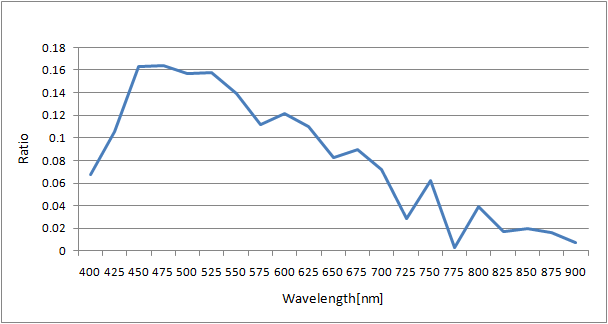
\includegraphics[scale=1]{chapters/img/wavelength_estimation.png}
\caption{Ratio of atmospheric transmittance versus photon detection efficiency}
\label{fig:wavelength_estimation}
\end{figure}
